\section{Analysis techniques}
\label{sec:method} 
 
\subsection{Power spectrum estimator}
The pseudo angular power spectrum \citep{hivon2002master} is utilized to extract information from the galaxy density contrast field, $\delta_{g}$, 
\begin{align}\label{eq:delta}
    \delta_{g} &= \frac{\rho- \overline{\rho}}{\overline{\rho}},
\end{align}
by decomposing it into spherical harmonics, $Y_{\ell m}$,
\begin{equation}
        a_{\ell m} = \int d\Omega ~ \delta_{g} W Y^{*}_{\ell m}.
\end{equation}
The mean galaxy density $\overline{\rho}$ is estimated from the entire LRG sample\footnote{The mean galaxy density is calculated separately for each region when we fit the power spectrum from each region individually.} and the survey window $W$ is determined from the number of randoms relative to the expected density of $6000$ randoms per square degrees. Then, the angular power spectrum is estimated by
\begin{equation}\label{eq:pusedocell}
        \tilde{C}_{\ell} = \frac{1}{2\ell +1} \sum_{m=-\ell}^{\ell} |a_{\ell m}|^{2}.
\end{equation}

We use the implementation of \texttt{anafast} from the \textsc{HEALPix} package \citep{gorski2005healpix} to do fast harmonic transforms and estimate the pseudo angular power spectrum and cross power spectrum. When the sky coverage of a survey is incomplete, this estimator yields a biased power spectrum. Specifically, the survey mask causes correlations between different harmonic modes and results in the measured power on scales near the survey size being pushed towards zero. Since these scales are highly sensitive to local primordial non-Gaussianity, it is crucial to account for these systematic effects in the model galaxy power spectrum to obtain unbiased $\fnl$ constraints.

 \subsection{Modeling}

\subsubsection{Angular power spectrum}
The relationship between the linear matter power spectrum $P(k)$ and the projected angular power spectrum of galaxies is expressed by the following equation:
\begin{equation}\label{eq:cell}
C_{\ell} = \frac{2}{\pi}\int_{0}^{\infty}\frac{dk}{k}k^{3}P(k)|\Delta_{\ell}(k)|^{2} + N_{\rm shot},
\end{equation}
where $N_{\rm shot}$ is a shot noise term that is not dependent on scale. The projection kernel $\Delta_{\ell}(k) = \Delta^{\rm g}_{\ell}(k) + \Delta^{\rm RSD}_{\ell}(k)$ includes redshift space distortions and determines the contribution of each wavenumber $k$ to the galaxy power spectrum on mode $\ell$. For more details, refer to \cite{Padmanabhan2007}. The FFTLog\footnote{\href{https://github.com/xfangcosmo/FFTLog-and-beyond}{github.com/xfangcosmo/FFTLog-and-beyond}} algorithm and its extension as implemented in \cite{fang2020beyond} are employed to calculate the integrals for the projection kernel $\Delta_{\ell}(k)$, which includes the $l^{\rm th}$ order spherical Bessel functions, $ j_{\ell}(kr)$, and its second derivatives,
\begin{align}
    \Delta^{\rm g}_{\ell}(k) &= \int \frac{dr}{r} r (b+\Delta b) D(r) \frac{dN}{dr} j_{\ell}(kr),\\
    \Delta^{\rm RSD}_{\ell}(k) &= - \int \frac{dr}{r} r f(r) D(r) \frac{dN}{dr} j^{\prime\prime}_{\ell}(kr),
\end{align}
where $b$ is the linear bias (dashed curve in Figure \ref{fig:nz}), $D$ represents the linear growth factor normalized as $D(z=0)=1$, $f(r)$ is the growth rate, and $dN/dr$ is the redshift distribution of galaxies normalized to unity and described in terms of comoving distance\footnote{$dN/dr = (dN/dz)*(dz/dr) \propto (dN/dz)*H(z)$} (solid curve in Figure \ref{fig:nz}). The PNG-induced scale-dependent shift is given by \citep{slosar2008constraints}
\begin{equation}
\Delta b = b_{\phi}(z) \fnl \frac{3 \Omega_{m} H^{2}_{0}}{2 k^{2}T(k)D(z) c^{2}} \frac{g(\infty)}{g(0)},
\label{eq:scaledepbias}
\end{equation}
where $\Omega_{m}$ is the matter density, $H_{0}$ is the Hubble constant\footnote{$H_{0}=100~({\rm km}~{\rm s}^{-1})/(h^{-1}{\rm Mpc})$ and $k$ is in unit of $h {\rm Mpc}^{-1}$}, $T(k)$ is the transfer function, and $g(\infty)/g(0) \sim 1.3$ with $g(z)\equiv (1+z) D(z)$ is the growth suppression due to non-zero $\Lambda$ and induced by our normalization of $D$ \citep[see, e.g.,][]{2010JCAP...07..013R, 2019MNRAS.485.4160M}. The bias parameter $b_{\phi}$ describes the response of galaxy formation to primordial potential perturbations in the presence of local PNG. Assuming that only mass determines the halo occupation function, $b_{\phi} = 2 \delta_{c}(b - p)$, where $p=1$ and $\delta_{c}= 1.686$ is the critical density for spherical collapse \citep{fillmore1984self}. The theoretical uncertainty on $p$ is not very well constrained, and \cite{2022JCAP...11..013B} showed that marginalizing over this parameter even with wide priors leads to biased $\fnl$ constraints because of parameter space projection effects. \cite{2023JCAP...01..023L} used N-body simulations to investigate secondary halo properties, such as concentration, spin and sphericity of haloes, and found that halo spin and sphericity preserve the universality of the halo occupation function while halo concentration significantly alters the halo function. Without better-informed priors on $p$, it is argued that the scale-dependent bias effect can only  be used to constrain the $b_{\phi}\fnl$ term \citep[see, e.g.,][]{2020JCAP...12..013B, 2020JCAP...12..031B}. However, the detection significance of local PNG remains unaffected by various assumptions regarding $p$. This means that a nonzero detection of $b_{\phi}\fnl$ at a certain confidence level will still indicate a nonzero detection of $\fnl$ at that same confidence level. This paper is focused on how a careful assessment of imaging systematic effects, or lack thereof, can bias our PNG constraints. Therefore, we choose $p=1$ for our sample of DESI LRG targets \citep[see, also,][]{slosar2008constraints,2010JCAP...07..013R,2013MNRAS.428.1116R}, and do not marginalize over $p$ to avoid projection effects \citep{2022JCAP...11..013B}.

\subsubsection{Survey geometry and integral constraint}
The ensemble average for the partial sky power spectrum is related to that of the full sky power spectrum via a mode-mode coupling matrix, $M_{\ell \ell^{\prime}}$,
\begin{equation}\label{eq:mixm}
    <\tilde{C}_{\ell}> = \sum_{\ell^{\prime}} M_{\ell \ell^{\prime}}<C_{\ell^{\prime}}>.
\end{equation}
In general, $M_{\ell \ell^{\prime}}$ is singular for a large footprint, but a common technique to remedy this issue is to use a discrete set of $\ell$ bins and assume that the angular power spectrum is constant in each bin. We follow a similar approach to \cite{chon2004fast} to do the convolution in Equation \ref{eq:mixm}. The theoretical galaxy power spectrum $C_{\ell}$ is convolved with the survey mask power spectrum to obtain the expected pseudo-power spectrum. The convolution in the spherical harmonics space becomes a multiplication in the correlation function space. First, we estimate the survey mask correlation function, $\hat{\omega}^{\rm window}$, and multiply that by the model correlation function, $\hat{\omega}^{\rm model}$. Then, the model pseudo-power spectrum is given by
\begin{align}
    \tilde{C}^{\rm model}_{\ell} &= 2\pi \int \hat{\omega}^{\rm model}\hat{\omega}^{\rm window}~P_{\ell}(\cos \theta) d\theta.
\end{align}

 \begin{figure}
\centering
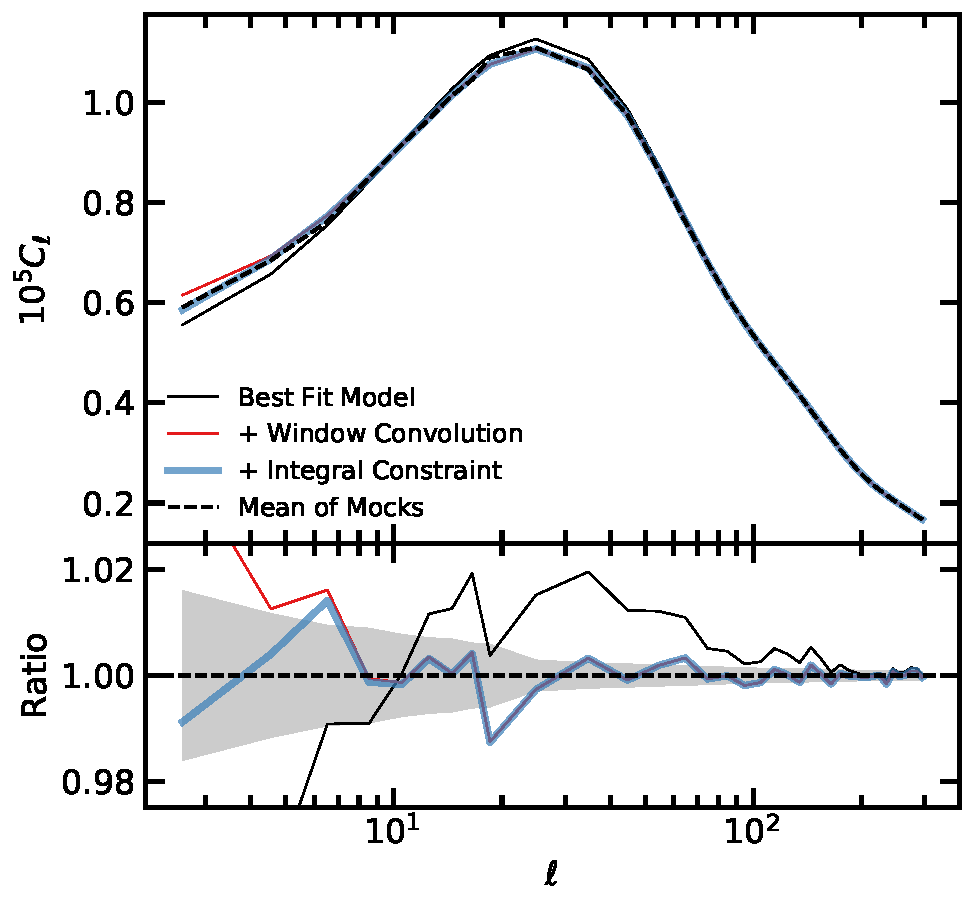
\includegraphics[width=0.45\textwidth]{model_mock.pdf}
\caption{The mean power spectrum from the $\fnl=0$ mocks (no contamination) and best fit theoretical prediction after accounting for the survey geometry and integral constraint effects. The dark and light shades represent $1\sigma$ error on the mean and one realization, respectively. Bottom panel shows the residual power spectrum relative to the mean power spectrum. No imaging systematic cleaning is applied to these mocks.}\label{fig:model_mock}
\end{figure}

The integral constraint is another systematic effect which is induced because the mean galaxy density is estimated from the observed galaxy density. The estimate of the mean density is biased by the limited sky coverage. This issue was first raised in \cite{peacock1991large}. To account for the integral constraint, the survey mask power spectrum is used to introduce a scale-dependent correction factor that needs to be subtracted from the power spectrum. Finally, the pseudo power spectrum with the integral constraint correction is obtained as
\begin{equation}
     \tilde{C}^{\rm model, IC}_{\ell} = \tilde{C}^{\rm model}_{\ell} - \tilde{C}^{\rm model}_{\ell=0} \left(\frac{\tilde{C}^{\rm window}_{\ell}}{\tilde{C}^{\rm window}_{\ell=0}}\right),
\end{equation}
where $\tilde{C}^{\rm window}$ is the spherical harmonic transform of $\hat{\omega}^{\rm window}$.

The lognormal simulations are used to validate our survey window and integral constraint correction. Figure \ref{fig:model_mock} shows the mean power spectrum of the $\fnl=0$ simulations (dashed) and the best fit theory prediction before and after accounting for the survey mask and integral constraint. The simulations are neither contaminated nor mitigated. The light and dark shades represent the 68\% estimated error on the mean and one single realization, respectively. The DESI mask is applied to the simulations, which covers around $40\%$ of the sky. We find that the survey window effect affects the clustering power on $\ell < 200$ and the integral constraint modulates the clustering power on $\ell < 6$.

\subsection{Parameter estimation}
Our parameter inference uses standard MCMC sampling. A constant clustering amplitude is assumed for the linear bias of our DESI LRG targets, $b(z) = b/D(z)$. In MCMC, we allow $\fnl$, $N_{\rm shot}$, and $b$ to vary, while all other cosmological parameters are fixed at the fiducial values (see \S \ref{ssec:mocks}). The galaxy power spectrum is divided into a discrete set of bandpower bins with $\Delta\ell=2$ between $\ell=2$ and $20$ and $\Delta \ell=10$ from $\ell=20$ to $300$. Each clustering mode is weighted by $2\ell+1$ when averaging over the modes in each bin.

With the lognormal simulations, we find that the distribution of the power spectrum at the lowest bin, $2\leq \ell < 4$, is asymmetric and its standard deviation varies significantly from the simulations with $\fnl=0$ to those with $76.9$ (Figure \ref{fig:histcell}). Therefore, we attempt to fit the log transformed power spectrum, $\log C_{\ell}$, to make our $\fnl$ constraints less sensitive to the choice of covariance matrix. The parameter $\fnl$ is constrained by minimizing a negative likelihood defined as,
\begin{equation}
-2\ln\mathcal{L} = (\log \tilde{C}(\Theta)-\log \tilde{C})^{\dagger} \mathbb{C}^{-1} (\log \tilde{C}(\Theta)-\log \tilde{C}),
\end{equation}
where $\Theta$ represents a container for the parameters $\fnl$, $b$, and $N_{\rm shot}$; $\tilde{C}(\Theta)$ is the (binned) expected pseudo-power spectrum; $\tilde{C}$ is the (binned) measured pseudo-power spectrum; and $\mathbb{C}$ is the covariance matrix constructed from the lognormal simulations. Flat priors are implemented for all parameters.

\begin{figure*}
\centering
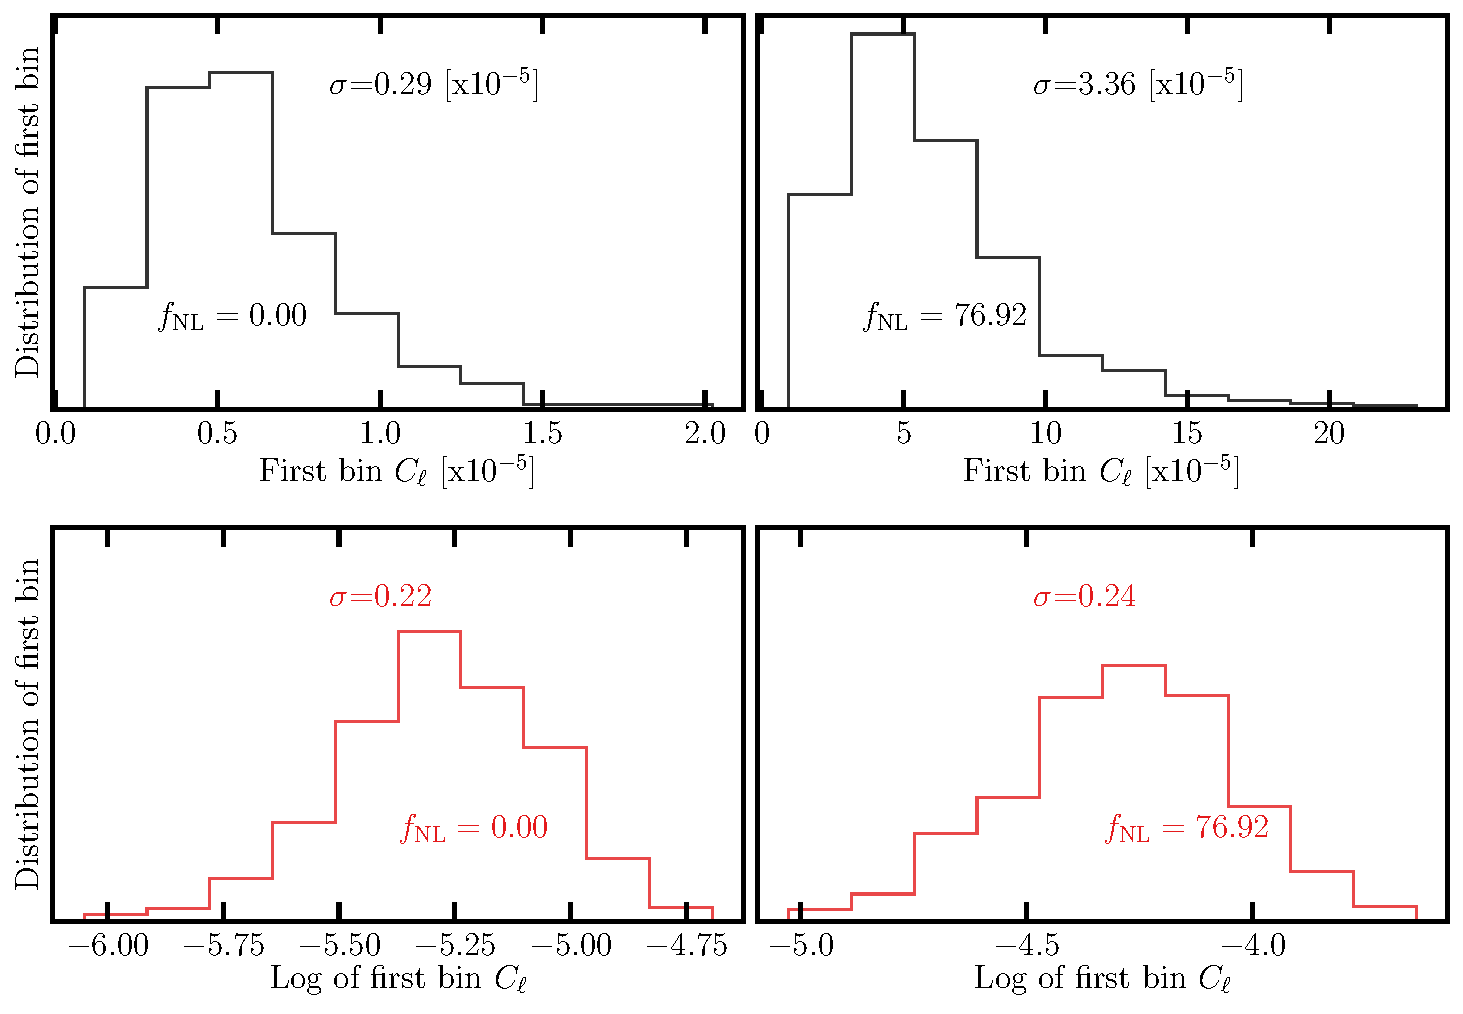
\includegraphics[width=0.85\textwidth]{hist_cl.pdf}
\caption{The distribution of the first bin power spectra and its log transformation from the simulations with $\fnl=0$ (left) and $76.92$ (right). The log transformation alleviates the asymmetry in the distributions.}\label{fig:histcell}
\end{figure*}


\subsection{Characterization of remaining systematics}
\label{ssec:characterization}

In the absence of systematic effects, a) the mean galaxy density should be uniform across the footprint within the statistical fluctuations regardless of imaging conditions and b) the cross power spectrum between the galaxy density and the imaging systematic maps should be consistent with zero within the statistical fluctuations. In the following, two statistical tests are implemented and applied to quantify remaining systematic effects in our sample \cite[see, also,][]{rezaie2021primordial}.

\begin{figure*}
\centering
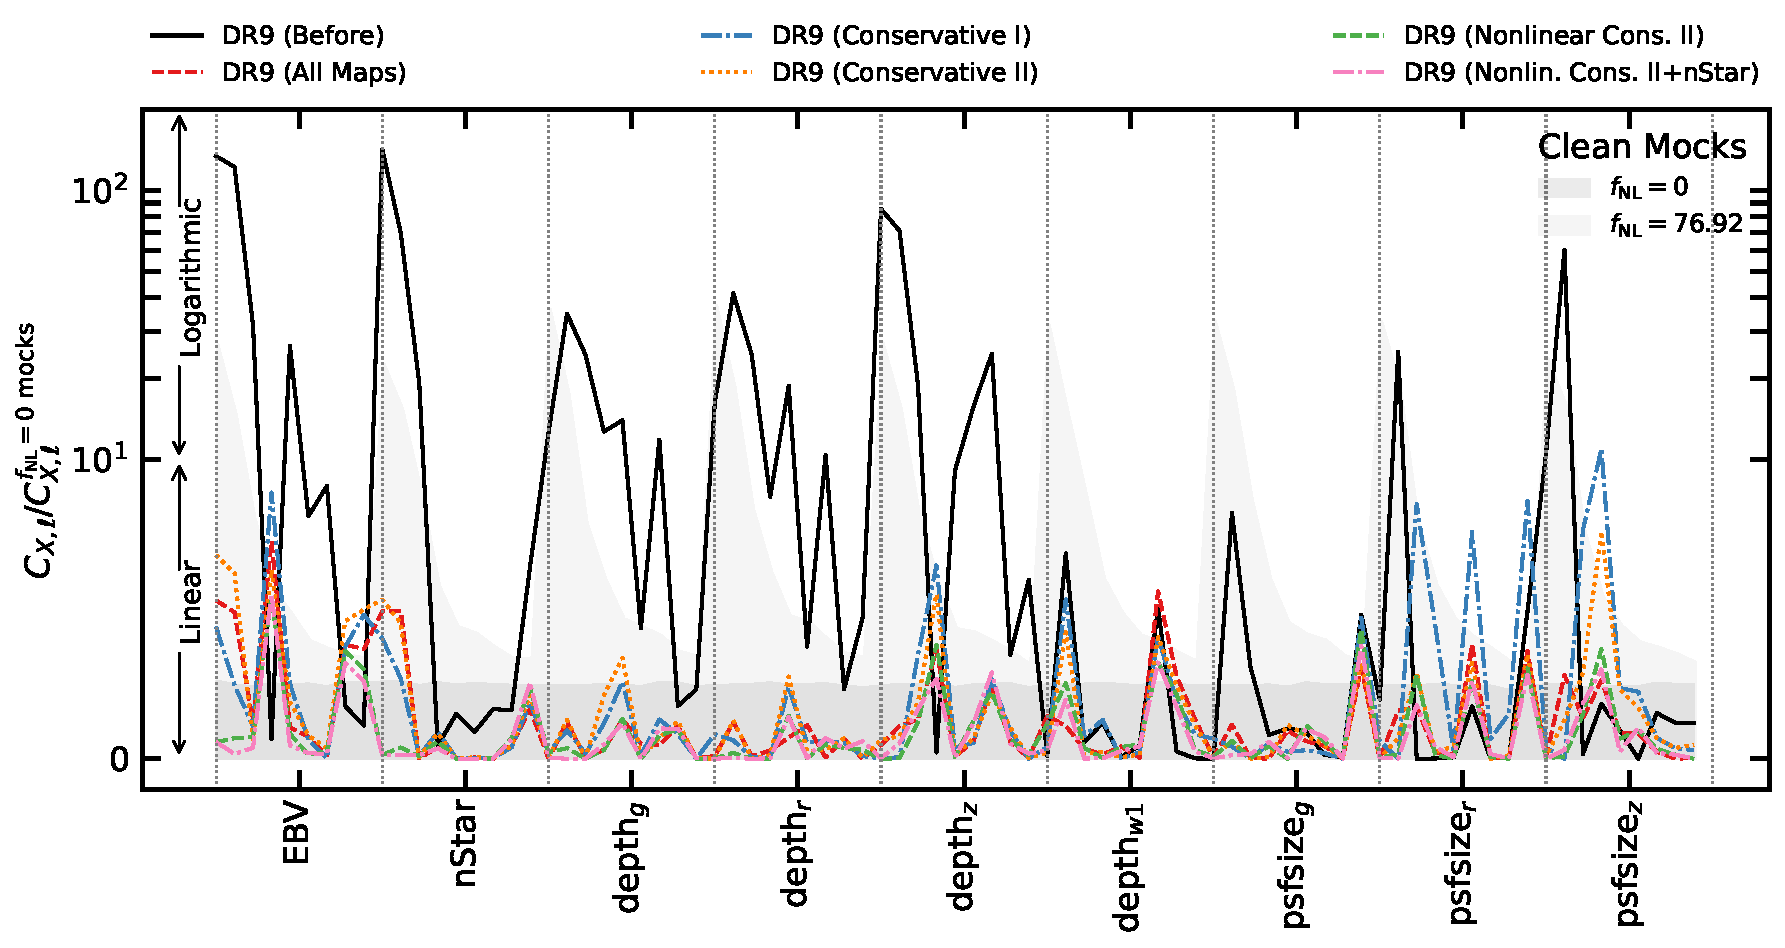
\includegraphics[width=0.95\textwidth]{clx_mocks.pdf}
\caption{The cross power spectra between the DR9 LRG sample and imaging systematic maps: Galactic extinction (EBV), stellar density (nStar), depth in \textit{grzw1} (depth$_{grzw1}$), and seeing in \textit{grz} (psfsize$_{grz}$). The black curves display the cross spectra before imaging systematic correction. The red, blue and orange curves represent the results after applying the imaging weights from the linear models trained with \textit{eight maps}, \textit{two maps}, and \textit{three maps}. The green and pink curves display the results after applying the imaging weights from the nonlinear models trained with \textit{three maps} and \textit{four maps}. The dark and light shades represent the $97.5$ percentile from cross correlating the imaging systematic maps and the $\fnl=0$ and $76.9$ lognormal density fields, respectively.}\label{fig:clxmock}
\end{figure*}

\begin{figure*}
\centering
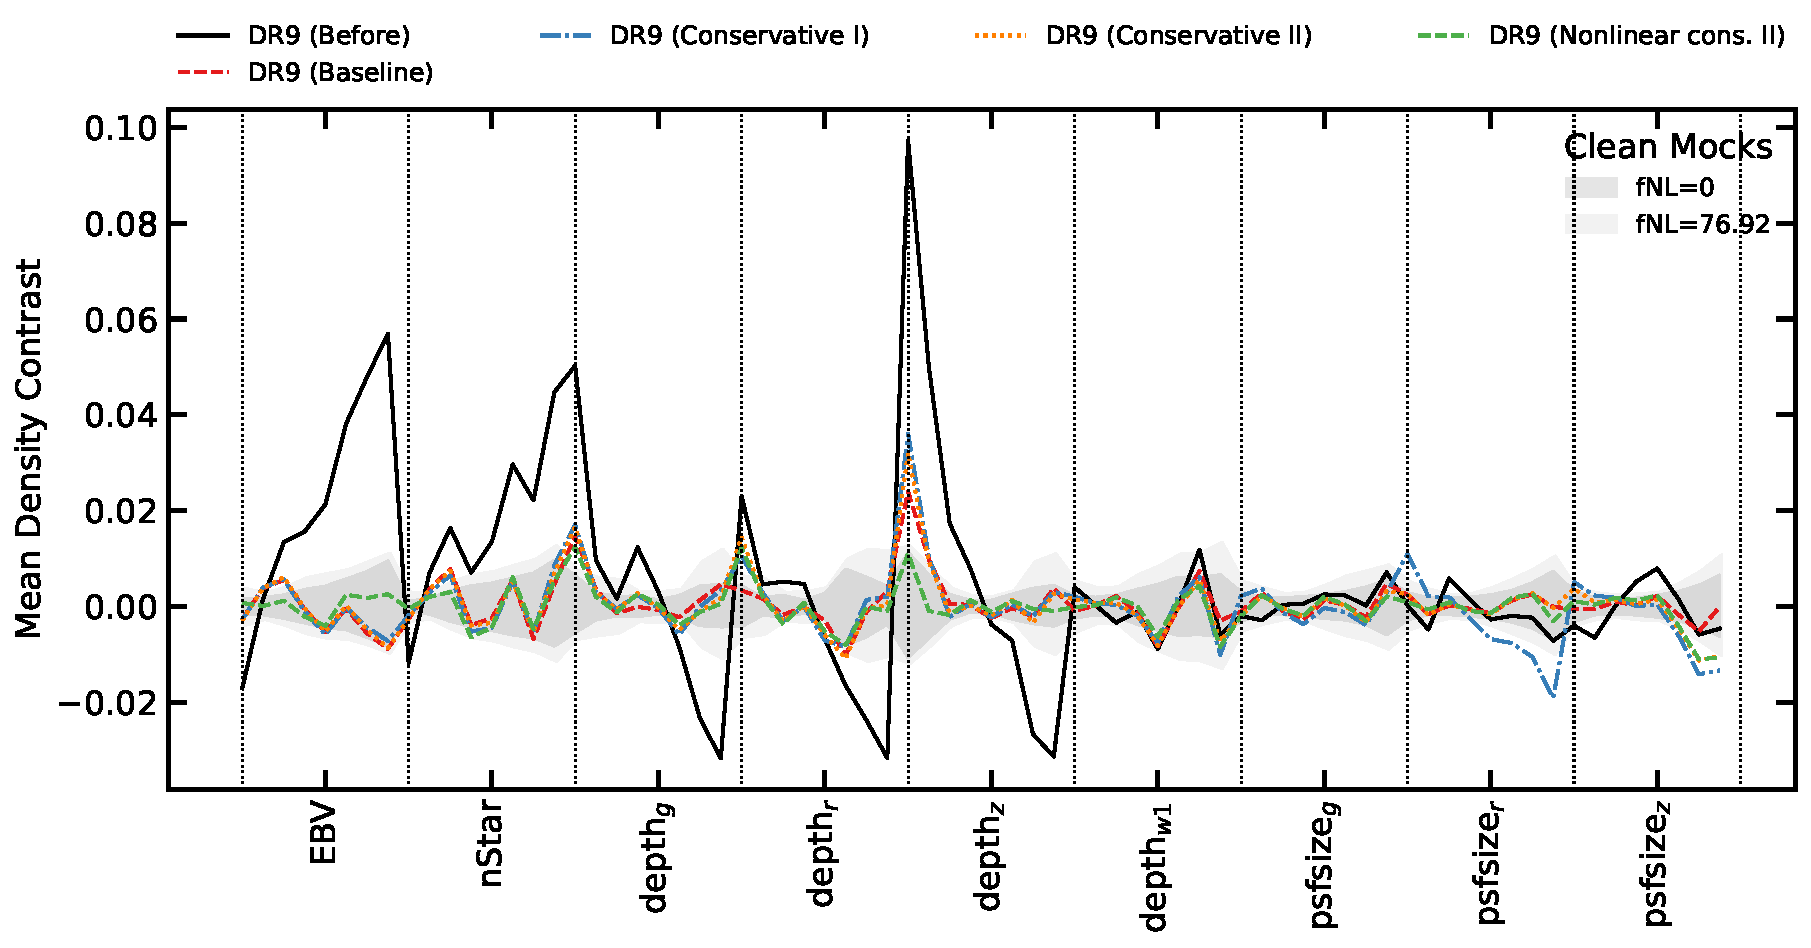
\includegraphics[width=0.95\textwidth]{nbar_mocks.pdf}
\caption{The mean density contrast of the DR9 LRG sample as a function of the imaging systematic maps: Galactic extinction (EBV), stellar density (nStar), depth in \textit{grzw1} (depth$_{grzw1}$), and seeing in \textit{grz} (psfsize$_{grz}$). The black curves display the results before imaging systematic correction. The red, blue and orange curves represent the relationships after applying the imaging weights from the linear models trained with \textit{eight maps}, \textit{two maps}, and \textit{three maps}. The green and pink curves display the results after applying the imaging weights from the nonlinear models trained with \textit{three maps} and \textit{four maps}. The dark and light shades represent the $1\sigma$ dispersion of 1000 lognormal mocks with $\fnl=0$ and $76.92$, respectively.}\label{fig:nbarmock}
\end{figure*}


\begin{figure}
\raggedleft
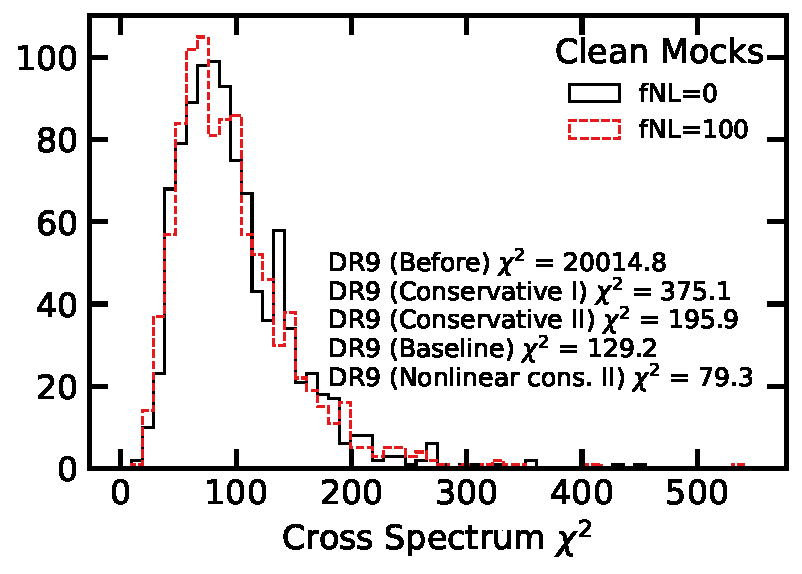
\includegraphics[width=0.45\textwidth]{chi2test.pdf}
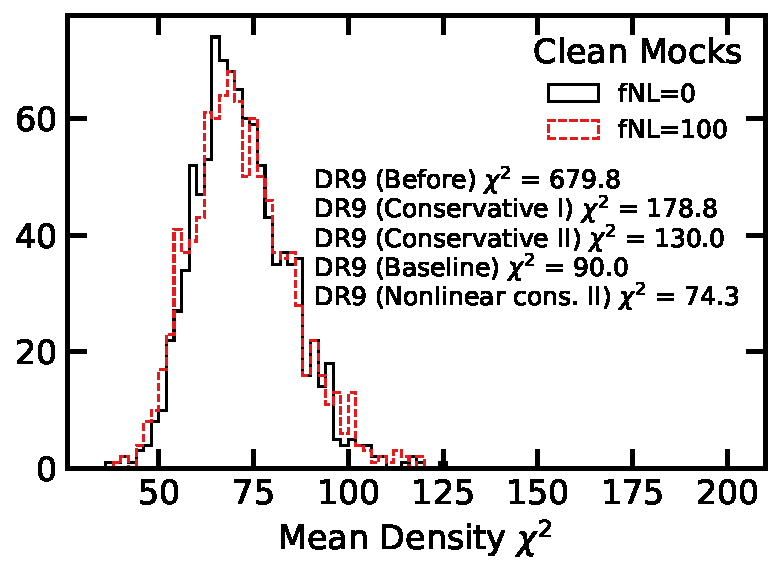
\includegraphics[width=0.44\textwidth]{chi2test2.pdf}
\caption{The remaining systematic error $\chi^{2}$ from the galaxy-imaging cross power spectrum (top) and the mean galaxy density contrast (bottom). The values observed in the DR9 LRG sample before and after linear and nonlinear treatments are quoted, and the histograms are constructed from 1000 realizations of clean lognormal mocks with $\fnl=0$ and $76.92$. \mr{Alex: can you show the DR9 chi2s as vertical lines rather than as text?}}\label{fig:chi2test}
\end{figure}


\subsubsection{Cross power spectrum}

We calculate the cross power spectra between the galaxy density and imaging \mr{systematic} maps \bbk{[Could we call them something else here (maybe contaminant maps)? I first got confused and thought you were cross-correlating redshift slices in your imaging survey, but maybe our readers will read more carefully than me]},
\begin{equation}
\tilde{C}_{X, \ell} = [\tilde{C}_{x_{1}, \ell}, \tilde{C}_{x_{2}, \ell}, \tilde{C}_{x_{3}, \ell}, ..., \tilde{C}_{x_{9}, \ell}],
\end{equation}
where $\tilde{C}_{x_{i}, \ell}$ represents the cross power spectrum between the galaxy density and $i^{\rm th}$ imaging map, $x_{i}$, normalized by the auto power spectrum of $x_{i}$:
\begin{equation}
\tilde{C}_{x_{i}, \ell} = \frac{(\tilde{C}_{gx_{i}, \ell})^{2}}{\tilde{C}_{x_{i}x_{i},\ell}}.
\end{equation}
Then, the $\chi^{2}$ value for the cross power spectra is calculated via,
\begin{equation}
\chi^{2} = \tilde{C}^{T}_{X, \ell} \mathbb{C}_{X}^{-1} \tilde{C}_{X, \ell},
\end{equation}
where the covariance matrix $\mathbb{C}_{X} = < \tilde{C}_{X, \ell} \tilde{C}_{X, \ell'} >$ is constructed from the lognormal mocks. These $\chi^{2}$ values are measured for every mock realization with the \textit{leave-one-out} technique and compared to the values observed in the DR9 sample with various imaging systematic corrections. Specifically, we use 999 realizations to estimate a covariance matrix and then apply the covariance matrix from the 999 realizations to measure the $\chi^{2}$ for the one remaining realization. This process is repeated for all 1000 realizations to construct a histogram for $\chi^{2}$. \bbk{[Can you elaborate a more what you mean by that?]}\mr{[MR: How is it now?]} We only include the bandpower bins from $\ell=2$ to $20$ with $\Delta\ell=2$, and test for the robustness with higher $\ell$ modes in Appendix \ref{sec:scalesys}. 

Figure \ref{fig:clxmock} shows $\tilde{C}_{X}$ from the DR9 LRG sample before and after applying various corrections for imaging systematics. The dark and light shades show the 97.5$^{\rm th}$ percentile from the $\fnl=0$ and $76.9$ mocks, respectively. The LRG sample has the highest cross-correlations against extinction, stellar density, and the z-band depth (solid black curve). As the most conservative cleaning approach, a linear model is trained with the extinction and z-band depth maps (\textit{linear two maps}) to derive the imaging systematic weights. With the correction applied, we find that the cross power spectrum against the r-band psfsize increases (dot-dashed blue curve), which indicates that only extinction and depth in the z-band are not sufficient to regress out all of the residual cross correlations between the LRG density and imaging. With the linear model re-trained using the three maps (\textit{linear three maps}), we are able to reduce the cross power spectra (dotted orange curve). For comparison, we also show the cross spectra for a case in which the DR9 is cleaned using the linear model trained with all imaging systematic maps (dashed red curve). There are minor differences between the \textit{linear three maps} and \textit{linear eight maps} cross spectra, further supporting the idea that only three imaging systematic maps are sufficient to regress out spurious correlations.

Figure \ref{fig:chi2test} (top) \bbk{[Figure 7 hasn't been discussed yet]} shows the histogram of the cross spectrum $\chi^{2}$ from 1000 mocks with and without $\fnl$. The $\chi^{2}$ values observed in the DR9 LRG sample are quoted for comparison. Before cleaning, our LRG sample has a cross power spectrum $\chi^{2}$ error of $20014.8$. After correction with the linear two maps approach, the cross spectrum $\chi^{2}$ is reduced to $375.1$ with p-value $=0.002$. Adding the r-band psfsize, the linear model reduces the $\chi^{2}$ down to $195.9$ with p-value $=0.044$; we can reject the null hypothesis that the DR9 sample with the linear three maps is properly cleaned at $95\%$ confidence. Even though training the linear model with all imaging systematic maps as input gives the lowest cross spectrum $\chi^{2}$ of $129.2$ (and p-value $=0.239$), it potentially makes the analysis more prone to over-fitting and regressing out the true clustering signal, given the inner correlations among the imaging properties (Figure \ref{fig:pcc}). As an alternative, we apply the imaging weights from the nonlinear method with the extinction, z-band depth, and r-band psfsize maps (\textit{nonlinear three maps}). The cross power spectrum $\chi^{2}$ is reduced to $79.3$ with p-value $=0.594$.  Adding the stellar density map reduces the cross power spectrum $\chi^{2}$ error to $70.9$ (p-value $=0.687$). Our cross power spectrum diagnostic supports the idea that a nonlinear cleaning approach is needed to properly regress out the remaining spurious fluctuations. We investigate the test with the cross power spectrum up to higher multipoles but find no evidence of remaining systematic errors (see Appendix \ref{sec:scalesys}). 

\subsubsection{Mean density contrast}
We calculate the histogram of the mean density contrast relative to the $j^{\rm th}$ imaging property:
\begin{equation}
\delta_{x_{j}} = ({\hat{\overline{\rho}}})^{-1} \frac{\sum_{i} \rho_{i} f_{{\rm pix}, i}}{\sum_{i} f_{{\rm pix}, i}},
\end{equation}
where the summations are over \textsc{HEALPix} pixels in the bin with similar imaging values. For instance, in the absence of systematic error, the mean density contrast from one part of the sky with high extinction should be consistent with that from another patch with low extinction. We compute the histograms against all other imaging properties (see Figure \ref{fig:ng}), and construct the total mean density contract as,
\begin{equation}
\delta_{X} = [\delta_{x_{1}}, \delta_{x_{2}}, \delta_{x_{3}}, ..., \delta_{x_{9}}],
\end{equation}
and the total residual error as,
\begin{equation}
\chi^{2} = \delta_{X}^{T} \mathbb{C_{\delta}}^{-1} \delta_{X},
\end{equation}
where the covariance matrix $\mathbb{C}_{\delta} = < \delta_{X} \delta_{X}>$ is constructed from the lognormal mocks. Figure \ref{fig:nbarmock} shows the mean density contrast against the imaging properties for the DR9 LRG sample. The dark and light shades represent the $1\sigma$ level fluctuations observed in 1000 lognormal density fields respectively with $\fnl=0$ and $76.92$. The DR9 LRG sample before treatment (solid curve) exhibits a strong trend around $10\%$ against the z-band depth which is consistent with the cross power spectrum. Additionally, there are significant spurious trends against extinction and stellar density at about $5-6\%$. The linear approach is able to mitigate most of the systematic fluctuations with only extinction and depth in the z-band as input; however,  a new trend appears against the r-band psfsize map with the \textit{linear two maps} approach (dot-dashed blue curve), which is indicative of the psfsize-related systematics in our sample. This finding is in agreement with the cross power spectrum. We re-train the linear model with three maps, but we still observe around $2\%$ residual spurious fluctuations in the low end of the z-band depth, which implies nonlinear systematic effects exist. We find that the imaging weights from the nonlinear model trained with the three identified maps (or four maps including the stellar density) is capable of reducing the fluctuations below $2\%$. We experiment with different binning schemes but find consistent results.

Figure \ref{fig:chi2test} (bottom) shows the mean density $\chi^{2}$ observed in the mocks with or without $\fnl$. We find consistent results regardless of the underlying $\fnl$, which supports that our diagnostic is not sensitive to the fiducial cosmology. The values measured in the DR9 LRG sample before and after applying imaging weights are quoted for comparison. The \textit{linear two maps} weights reduce the $\chi^{2}$ value from $679.8$ (before correction) to $178.8$. The p-value $=0$ indicates severe remaining systematic effects. Adding the r-band psfsize does not reduce the p-value enough (e.g., greater than $0.05$) even though the cleaning method yields a lower $\chi^{2}=130$. Training the linear model with all imaging systematic maps returns a more reasonable $\chi^{2}=90$ and p-value of $0.084$. However, regression with all imaging systematic maps as input can lead to the removal of the true clustering signal. With the imaging weights from the \textit{nonlinear three maps} approach, we obtain a $\chi^{2}$ value of $74.3$ with p-value $=0.392$. Re-training the nonlinear approach while adding the stellar density map (\textit{nonlinear four maps}) yields minor improvement: $\chi^{2}=73.2$ and p-value $=0.422$.  This indicates that the stellar density trend in the mean LRG density can be explained via the extinction map.




\subsection{Calibration of mitigation bias}\label{ssec:calibration}
The template-based mitigation of imaging systematics removes some of the true clustering signal, and the amount of the removed signal increases as more maps are fed to the regression. Supported by our remaining systematic test, \textit{nonlinear three maps} is therefore chosen as our default approach and is applied to the mocks (with and without contaminations) to calibrate the $\fnl$ biases induced by over-correction. Below we describe an approach for the calibration and de-biasing of our $\fnl$ constraints. 

\begin{figure}
\centering
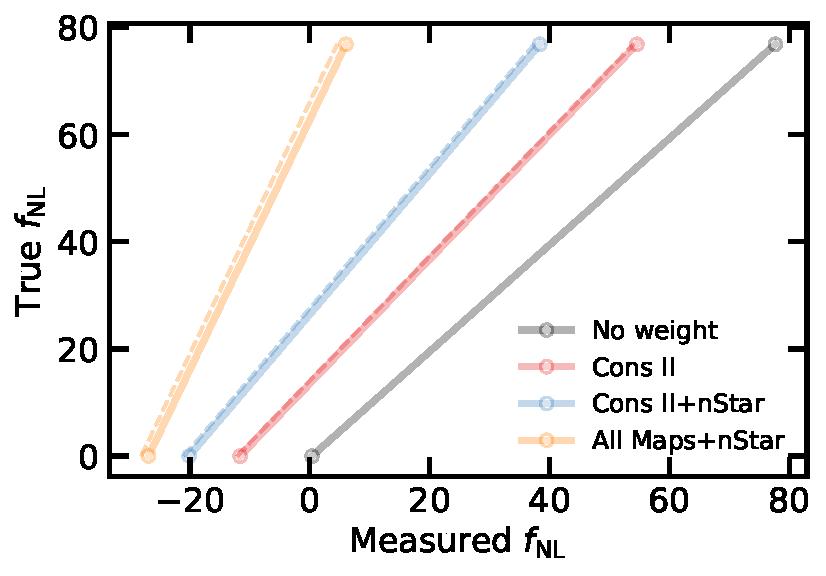
\includegraphics[width=0.45\textwidth]{figures/fnlbias}
\caption{The \textit{No mitigated, clean} vs \textit{mitigated} $\fnl$ values from the $\fnl=0$ and $76.9$ mocks. The solid (dashed) lines represent the best fit estimates from fitting the mean power spectrum of the clean (contaminated) mocks. The scatter points show the best fit estimates from fitting the individual spectra for the clean mocks.}\label{fig:fnlbias}
\end{figure}

To calibrate for over-correction, we utilize our series of lognormal density fields with and without PNG, with and without systematic effects. The contamination model is based on the linear multivariate approach with the extinction, z-band depth, and r-band psfsize maps as input and parameters drawn from the likelihood constrained by the DR9 LRG sample. The idea is to simulate systematic effects that reflect spurious fluctuations as  realistic as the DR9 LRG sample. For correction, the neural network model is trained and applied to the simulations with various sets of imaging systematic maps as input. Particularly, we consider \textit{nonlinear three maps}, \textit{nonlinear four maps}, and \textit{nonlinear nine maps}. We fit both the mean power spectrum and each individual power spectrum of 1000 realizations. The best fit estimates from the mocks without systematics (and no mitigation applied) are considered as the true $\fnl$ values and the estimates from the mocks (with the mitigation procedure applied) are considered as the measured $\fnl$ values. Figure \ref{fig:fnlbias} shows the true $\fnl$ values vs the measured $\fnl$ values from fitting the mean power spectrum (solid lines) and individual spectra (points). The dashed lines show the best fit estimates from the contaminated realizations. The best fit estimates for the contaminated mocks before cleaning (\textit{no weight}) or per realizations are not shown for visual clarity. 

Then, a pair of linear parameters are found to map the measured values to the true values, $f_{\rm NL, true} = m_{1} f_{\rm NL, measured} + m_{2}$. These $m_{1}$ and $m_{2}$ coefficients for the mean power spectrum are summarized in Table \ref{tab:debiasparams}. The coefficients for the \textit{nonlinear nine maps} approach are the highest, as more mitigation bias is expected if more imaging systematic maps are used. We find that $m_{1}-1$ determines the added uncertainty in the $\fnl$ constraints, once the correction coefficients are applied. We expect this effect to be maximum for \textit{nonlinear nine maps} and minimum for \textit{nonlinear three maps}.

\begin{table}
\begin{center}
\caption{Linear parameters employed to de-bias the $\fnl$ constraints to account for the over-correction issue.}\label{tab:debiasparams}
\begin{tabular}{lcc}
\hline
\hline
\textbf{Cleaning Method} & $m_{1}$ & $m_{2}$ \\
\hline
Nonlinear Three Maps & 1.17 & 13.95 \\
Nonlinear Four Maps & 1.32 & 26.97 \\
Nonlinear Nine Maps & 2.35 & 63.5\\
\hline
\end{tabular}
\end{center}
\end{table}